\section{Language Modeling}
Quando si lavora con un enorme corpus di dati testuali, è utile conoscere la probabilità con cui una sequenza di parole si succederà e quali particolari caratteristiche sono necessarie per capire questa dipendenza.

Il Language Modeling è il compito di capire questa distribuzione di probabilità su una sequenza di parole. Ciò aiuta a creare caratteristiche che possono distinguere tra frasi e frasi, secondo il contesto in cui appaiono.
I modelli linguistici interpretano questi dati alimentandoli attraverso un algoritmo che stabilisce regole per il contesto nel linguaggio naturale. A questo punto, il modello applica queste regole in compiti linguistici per prevedere o produrre nuove frasi. Il modello essenzialmente impara le caratteristiche del linguaggio di base e usa queste caratteristiche per capire nuove proposizioni.

Esistono diversi approcci probabilistici al language modeling, che variano a seconda dello scopo del modello linguistico. In questa tesi, è stato implementato un approccio al language modeling atto a modellare il testo in modo tale che questo possa essere convertito in un input numerico per una rete neurale artificiale. Nelle sezioni successive verrà approfondito proprio questo concetto, chiamato \textit{Word Embedding}, per poi discutere in particolar modo dei modelli \textit{GloVe}\textsuperscript{\cite{pennington-etal-2014-glove}}, \textit{BERT}\textsuperscript{\cite{devlin2019bert}} e \textit{USE}\textsuperscript{\cite{cer2018universal}}, utilizzati durante la fase di sperimentazione descritta nei capitoli successivi.
\subsection{Word Embedding}
Word embedding è il nome collettivo per definire un insieme di tecniche di language modeling e di apprendimento delle caratteristiche nell'elaborazione del linguaggio naturale in cui le parole o le frasi del vocabolario sono mappate in vettori di numeri reali. La necessità di questa pratica è nata con lo sviluppo delle reti neurali artificiali dato che, come accennato nella sezione riguardante il Deep Learning, esse possono elaborare soltanto input di natura numerica.

L'embedding si basa sul fatto che, in genere, le parole con un significato simile avranno rappresentazioni vettoriali che sono vicine tra loro nello spazio di incorporazione (anche se questo non è sempre stato il caso). Quando si codificano le parole, tipicamente l'obiettivo è quello di catturare qualche tipo di relazione in quello spazio, che sia il significato, la morfologia, il contesto o qualche altro tipo di connessione.

Molti word embedding sono creati sulla base della nozione introdotta dall'\textit{ipotesi distributiva} di Zellig Harris\textsuperscript{\cite{distributional_structure}}, che si riduce a una semplice idea che le parole che sono usate vicine l'una all'altra hanno tipicamente lo stesso significato.

Ciò diventa particolarmente utile quando i set di dati diventano sempre più grandi, perché con l’aumentare delle dimensioni spesso aumenta anche il numero di parole uniche. La presenza di molte parole usate raramente può causare problemi per un modello lineare; questo perché la quantità di possibili sequenze di parole aumenta, e i modelli che informano i risultati diventano più deboli. Ponderando le parole in modo non lineare e distribuito, questo modello può "imparare" ad approssimare le parole e quindi non essere fuorviato da eventuali valori sconosciuti. La sua "comprensione" di una data parola non è così strettamente legata alle parole immediatamente circostanti.

\subsection{Embedding statico: GloVe}
\textbf{GlobalVectors} (GloVe) è un modello assai noto che apprende i vettori o le parole dalle informazioni di co-occorrenza, ovvero la frequenza con cui compaiono insieme in grandi corpora di testo. GloVe è basato sul conteggio. In linea generale i modelli basati sul conteggio apprendono i vettori, operando una riduzione della dimensionalità sulla matrice di conteggio delle co-occorrenze.

Per prima cosa, si costruisce una grande \textbf{matrice di co-occorrenza} (parole x colonne), che contiene le informazioni sulla frequenza con cui ogni parola viene usata in un contesto. Il numero di contesti deve essere grande, poiché è essenzialmente di dimensioni combinatorie.

In seguito, tale matrice viene riscritta in forma algebrica e fattorizzata per ottenerne una dimensionalmente più piccola. Il risultato di questa operazione è una rappresentazione vettoriale per ogni parola.

L’addestramento può poi essere eseguito in due modi diversi: utilizzando il contesto per predire una parola target (utilizzando metodi noti come il BoW\textsuperscript{\cite{bow_article}} o il CBoW\textsuperscript{\cite{mikolov2013efficient}}) oppure usando una parola per predirre il contesto target (Skip-Gram\textsuperscript{\cite{skipgram}}).
% Precisamente, l'algoritmo GloVe consiste nei seguenti passi:
% \begin{enumerate}
%     \item Raccogliamo le statistiche di co-occorrenza delle parole in una forma di matrice di co-occorrenza di parole \(X\). Ogni elemento \(X_i_j\) di tale matrice rappresenta quanto spesso la parola \(i\) appare nel contesto della parola \(j\). Di solito scansioniamo il nostro corpus nel seguente modo: per ogni termine cerchiamo termini contestuali entro una certa area definita da una costante chiamata \(dimensione_finestra\) prima del termine e una \(dimensione_finestra\) dopo il termine. 
%     \clearpage
%     \begin{figure}[hbt!]
%         \centering
%         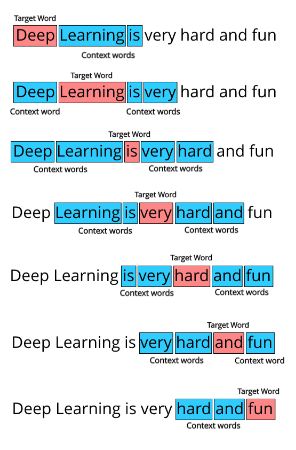
\includegraphics[width=0.5\textwidth]{img/context_window.png}
%         \caption{Context Window}
%         \label{fig:context_window}
%     \end{figure} \\
%     Inoltre diamo meno peso alle parole più lontane, di solito usando questa formula:
%     \begin{center}
%         \(decay=1/offset\)
%     \end{center}
    
%     \item Definiamo i vincoli per ogni coppia di parole:
%     \begin{center}
%         \(w^T_i w_j + b_i + b_j = log(X_i_j)\)
%     \end{center}
%     dove \(w_i\) è il vettore per la parola principale, \(w_j\) è il vettore per la \textit{context word}, \(b_j, b_j\) sono bias scalari rispettivamente per la parola principale e di contesto
    
%     \item Definiamo una funzione di costo:
%     \begin{center}
%         \[J = \sum_{i=1}^{V} \sum_{j=1}^{V} f(X_i_j)(w^T_i w_j + b_i + b_j - log(X_i_j))^2\]
%     \end{center}
%     Qui \(f\) è una funzione di ponderazione che ci aiuta a prevenire l'apprendimento solo da coppie di parole estremamente comuni. Gli autori di GloVe hanno scelto la seguente funzione:
%     \begin{center}
%         \[ f(X_i_j) = 
%           \begin{cases} 
%                 (\frac{X_i_j}{X_m_a_x})^\alpha & if X_i_j < X_m_a_x \\
%                 1 & otherwise
%             \end{cases}
%         \]
%     \end{center}
% \end{enumerate}
\subsection{Embedding contestualizzati: BERT}
I modelli statici come GloVe presentano diverse limitazioni:
\begin{itemize}
    \item L'uso di modelli linguistici molto superficiali. Questo significa che c'è un limite alla quantità di informazioni che possono catturare.
    \item Un'altra limitazione chiave è che questi modelli non prendono in considerazione il contesto della parola: questi modelli producono un solo embedding per ogni parola, combinando tutti i diversi sensi della parola in un unico vettore.
\end{itemize}
Alla fine del 2018 i ricercatori di Google AI Language hanno reso open-source una nuova tecnica per l'elaborazione del linguaggio naturale (NLP) chiamata \textbf{BERT (Bidirectional Encoder Representations from Transformers)} - una grande svolta che ha preso d'assalto la comunità del Deep Learning per le sue incredibili prestazioni. Il team di ricerca che ha lavorato dietro BERT lo descrive così:
\begin{center}
    \textit{"BERT sta per Bidirectional Encoder Representations from Transformers.  È progettato per pre-addestrare rappresentazioni bidirezionali profonde da testi non etichettati, condizionando congiuntamente il contesto sinistro e destro. Come risultato, il modello BERT pre-addestrato può essere messo a punto con un solo strato di output aggiuntivo per creare modelli all'avanguardia per una vasta gamma di compiti NLP."}
\end{center}
In primo luogo, BERT è basato sull'architettura \textbf{Transformer}, un modello proposto nel paper \textit{Attention is All You Need}\textsuperscript{\cite{vaswani2017attention}} che usa l'\textit{attenzione} (successore del modello sequence-to-sequence) per accelerare il processo di addestramento. In secondo luogo, BERT è pre-addestrato su un grande corpus di testo non etichettato che include l'intera \textbf{Wikipedia} (2.500 milioni di parole) e il Book Corpus (800 milioni di parole). In terzo luogo, BERT è un modello \textit{"profondamente bidirezionale"}. Bidirezionale significa che BERT apprende informazioni sia dal lato sinistro che da quello destro del contesto di un token durante la fase di formazione.

Il paper pubblicato dai creatori di Bert, presenta due modelli che si differenziano per le loro dimensioni: \begin{itemize}
    \item \textbf{BERT Base}: 12 strati (blocchi di trasformatori), 12 teste di attenzione e 110 milioni di parametri
    \item \textbf{BERT Large}: 24 strati (blocchi di trasformatori), 16 teste di attenzione e 340 milioni di parametri
\end{itemize}
\begin{figure}[hbt!]
    \centering
    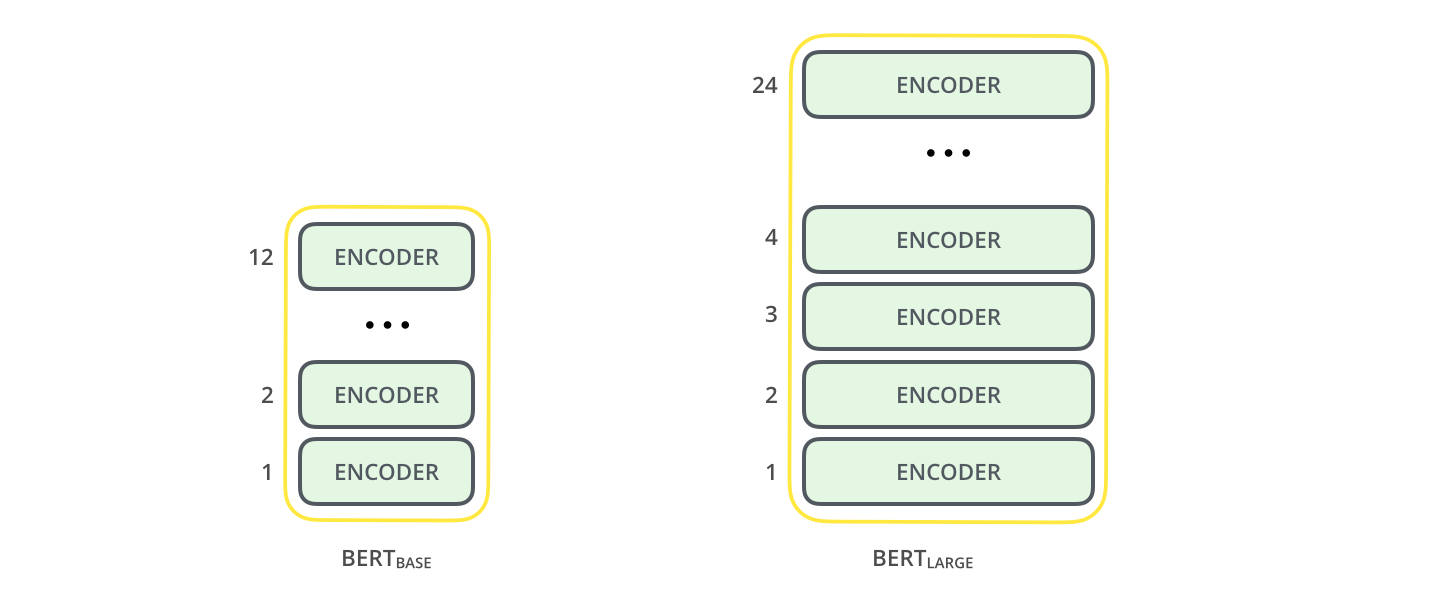
\includegraphics[width=1\textwidth]{img/bert_architecture.png}
    \caption{BERT Base e BERT Large}
    \label{fig:bert_architettura}
\end{figure}
\newpage
BERT è pre-addestrato su due compiti NLP:
\begin{itemize}
    \item \textbf{Masked Language Model}: Viene utilizzato per addestrare la capacità di BERT di catturare informazioni in maniera bidirezionale. Data una frase, il 15\% di essa viene \textit{mascherato} usando token speciali (ad esempio "[MASK]") e viene chiesto di prevedere la parola corretta che dovrebbe trovarsi in quella posizione. Durante l'addestramento di BERT viene utilizzata la seguente tecnica:
    \begin{enumerate}
        \item L'80\% delle volte le parole sono state sostituite con il token mascherato [MASK].
        \item Il 10\% delle volte le parole sono state sostituite con parole casuali.
        \item Il 10\% delle volte le parole sono rimaste invariate.
    \end{enumerate}
    \item \textbf{Next Sentence Prediction}: Questo è un task di classificazione binaria che viene utilizzato per addestrare BERT, in modo tale che quest'ultimo possa essere utilizzato in compiti nei quali è necessario sapere comprendere le relazioni che intercorrono tra le frasi. Il quesito posto è: date due frasi A e B prese da un corpus linguistico, determinare se la frase B segue la frase A nel testo oppure no.   
    \begin{enumerate}
        \item Per il 50\% delle coppie, la seconda frase sarebbe in realtà la frase successiva alla prima.
        \item Per il restante 50\% delle coppie, la seconda frase sarebbe una frase casuale dal corpus.
    \end{enumerate}
\end{itemize}
\subsection{Embedding contestualizzati: Universal Sentence Encoder}
BERT è uno strumento molto potente ma, proprio per questo motivo non è la soluzione migliore quando si tratta di utilizzarlo su dispositivi con memoria o potenza di calcolo limitata. È da questa idea che nasce il progetto proposto da \citet{cer2018universal}.

L'\textbf{Universal Sentence Encoder (USE)} codifica il testo in vettori ad alta dimensione che possono essere utilizzati per la classificazione del testo, la similarità semantica, il clustering e altri compiti del Natural Language Processing. L'idea è quella di progettare un codificatore che riassuma qualsiasi frase data in un'embedding a 512 dimensioni. Si usa questo stesso embedding per risolvere compiti multipli e in base agli errori che vengono fatti su di essi, aggiorniamo la codifica della frase. Poiché essa deve lavorare su più compiti generici, catturerà solo le caratteristiche più informative e scarterà il rumore. L'intuizione è che, così facendo, il risultato possa essere universalmente compatibile per essere incorporato a diversi task anche molto distanti tra loro.

L'Universal Sentence Encoder pre-addestrato è disponibile pubblicamente in \textbf{Tensorflow-hub}. Viene fornito in due varianti:
\begin{enumerate}
    \item \textbf{Transformer Encoder}: In questa variante, usiamo la parte encoder dell'architettura originale del transformer. L'architettura consiste di 6 strati di trasformatori impilati. Ogni strato ha un modulo di self-attention seguito da una rete feed-forward.
    \item \textbf{Deep Averaging Network}: Word embeddings e i bi-grammi presenti in una frase sono mediate insieme. Poi attraversano una DNN profonda a 4 strati feed-forward per ottenere in uscita un'embedding per l'intera frase a 512 dimensioni. Le embeddings per le parole e i bi-grammi sono apprese durante l'addestramento.
\end{enumerate}
I due modelli hanno un compromesso di accuratezza e richiesta di risorse computazionali. Mentre quello con un codificatore Transformer ha una maggiore precisione ma è computazionalmente più intenso, quello con codifica DAN usa meno memoria con un leggero compromesso a livello di precisione.

Il modello di codifica è progettato per essere il più generale possibile. Ciò viene realizzato utilizzando l'apprendimento multi-task in cui un singolo modello di codifica viene addestrato per risolvere più compiti diversi. I tasks supportati includono: un compito simile a Skip-Thought (\citet{NIPS2015_f442d33f}) per l'apprendimento non supervisionato da un testo corrente arbitrario; un task di input-risposta conversazionale (\citet{henderson2017efficient}); e compiti di classificazione per l'addestramento su dati supervisionati. Il compito Skip-Thought sostituisce il LSTM (\citet{Hochreiter1997LongSM}) usato nella formulazione originale con un modello un modello basato sull'architettura Transformer. 
